\documentclass[a4paper,titlepage,12pt]{article}
\usepackage[utf8]{inputenc} %Make sure all UTF8 characters work in the document
\usepackage{listings} %Add code sections
\usepackage{color}
\usepackage{graphicx}
\usepackage{titling}
\usepackage{textcomp}
\usepackage{tabularx}
\usepackage[hyphens]{url}
\usepackage[bottom]{footmisc}
\usepackage[yyyymmdd]{datetime}
\definecolor{listinggray}{gray}{0.9}
\definecolor{lbcolor}{rgb}{0.9,0.9,0.9}

%Set page size
\usepackage{geometry}
\geometry{margin=3cm}
\usepackage{parskip} 

\renewcommand{\dateseparator}{-}

%\author{
%    Emil Segerbäck - emise935
%    \and
%    Frans Skarman - frask812
%    \and
%    Hannes Tuhkala - hantu447
%    \and
%    Malcolm Vigren - malvi108
%    \and
%    Noak Ringman - noari093
%    \and
%    Olav Övrebö - olaov121
%    \and
%    Robin Sliwa - robsl733}


%%%%%%%%%%%%%%%%%%%%%%%%%%%%%%%
% Header and footer
%%%%%%%%%%%%%%%%%%%%%%%%%%%%%%%
\usepackage{fancyhdr}
\pagestyle{fancy}

\lhead{FIN LOGGA}
\chead{LiTHe Hex}
\rhead{\today}

\lfoot{TSEA29 - Konstruktion med mikrodatorer \\ LIPS Kravspecifikation}
\rfoot{Grupp 9}


\title{\textbf{Kravspecifikation}}
\date{\today}

\begin{document}
	\maketitle
	\newpage

	
	\begin{center}

		%%%%%%%%%%%%%%%%%%%%%%%%%%%%%%%%%%%%%%%%%%%%%%%%%%%%%%%%%%%%%%%%%%%%%%%%%%%%%%%%%
		%						Medlemmar
		%%%%%%%%%%%%%%%%%%%%%%%%%%%%%%%%%%%%%%%%%%%%%%%%%%%%%%%%%%%%%%%%%%%%%%%%%%%%%%%%%

		\section*{Projektidentitet}
		Grupp 9, Ht 2016, LiTHe Hex

		Linköpings tekniska högskola, ISY

		\begin{table}[h]
			\begin{tabular}[pos]{| l | l | l | l |}
				\hline
				\textbf{Namn} & \textbf{Ansvar} & \textbf{Telefon} & \textbf{E-Post} \\ \hline
				Frans Skarman & Dokumentansvarig & 0708798660 & frask812@student.liu.se \\ \hline
			\end{tabular}
		\end{table}


		Kundinfo?

		\textbf{Kursansvarig}: Tomas Svensson Rum 3B:528 013-28 13 68 tomas.svensson@liu.se

		\textbf{Handledare}:


		
		\newpage


		%%%%%%%%%%%%%%%%%%%%%%%%%%%%%%%%%%%%%%%%%%%%%%%%%%%%%%%%%%%%%%%%%%%%%%%%%%%%%%%%%
		%						Historik
		%%%%%%%%%%%%%%%%%%%%%%%%%%%%%%%%%%%%%%%%%%%%%%%%%%%%%%%%%%%%%%%%%%%%%%%%%%%%%%%%%

		\section*{Dokumenthistorik}
		\begin{table}[h]
			\begin{tabular}[pos]{| l | l | l | l | l |}
				\hline
				\textbf{Version} & \textbf{Datum} & \textbf{Utförda förändringar} 
				& \textbf{Utförda av} & \textbf{Granskad} \\ \hline

				0.1 & 2016-09-05 & Första utkastet & ckr & \\ \hline

			\end{tabular}
		\end{table}

	\end{center}

	%%%%%%%%%%%%%%%%%%%%%%%%%%%%%%%%%%%%%%%%%%%%%%%%%%%%%%%%%%%%%%%%%%%%%%%%%%%%%%%%%
	%						Inledning
	%%%%%%%%%%%%%%%%%%%%%%%%%%%%%%%%%%%%%%%%%%%%%%%%%%%%%%%%%%%%%%%%%%%%%%%%%%%%%%%%%

	\newpage

	\section{Inledning}
	I detta dokument kommer det att framgå vilken funktionalitet som produkten kommer 
	att ha vid leverans. All funktionalitet har strukturerats i olika krav där det 
	blir tydligt hur vida kravet är uppfyllt eller inte. Krav har olika nivåer där
	nivå 1 är se krav som måste ha uppfyllts vid leverans. Nivå 2 ses som bör krav 
	och uppfylls i mån om tid. Varje krav kommer att ha följande struktur. 
	\textbf{fin figur}

	\subsection{Parter}
	Projektet har parter som består av beställare/kund Tomas Svensson lektor vid 
	Linköpings tekniska högskola och producent projektgrupp 9 bestående av 7 
	studenter från D-programmet vid Linköpings tekniska högskola. 
	\subsection{Syfte och mål}
	Syftet och målet med projektet är att utveckla en sexbent robot som själv
	kan navigera sig ut ur en labyrint. I labyrinten ska roboten även kunna ta 
	sig över hinder för att komma vidare. 
	\subsection{Användning}
	\textbf{text}
	\subsection{Bakgrundsinformation}
	\textbf{text}
	\subsection{Definitioner}

	%%%%%%%%%%%%%%%%%%%%%%%%%%%%%%%%%%%%%%%%%%%%%%%%%%%%%%%%%%%%%%%%%%%%%%%%%%%%%%%%%
	%						Översikt
	%%%%%%%%%%%%%%%%%%%%%%%%%%%%%%%%%%%%%%%%%%%%%%%%%%%%%%%%%%%%%%%%%%%%%%%%%%%%%%%%%

	\section{Översikt av systemet}
	\begin{figure}[h!]
		\centering
		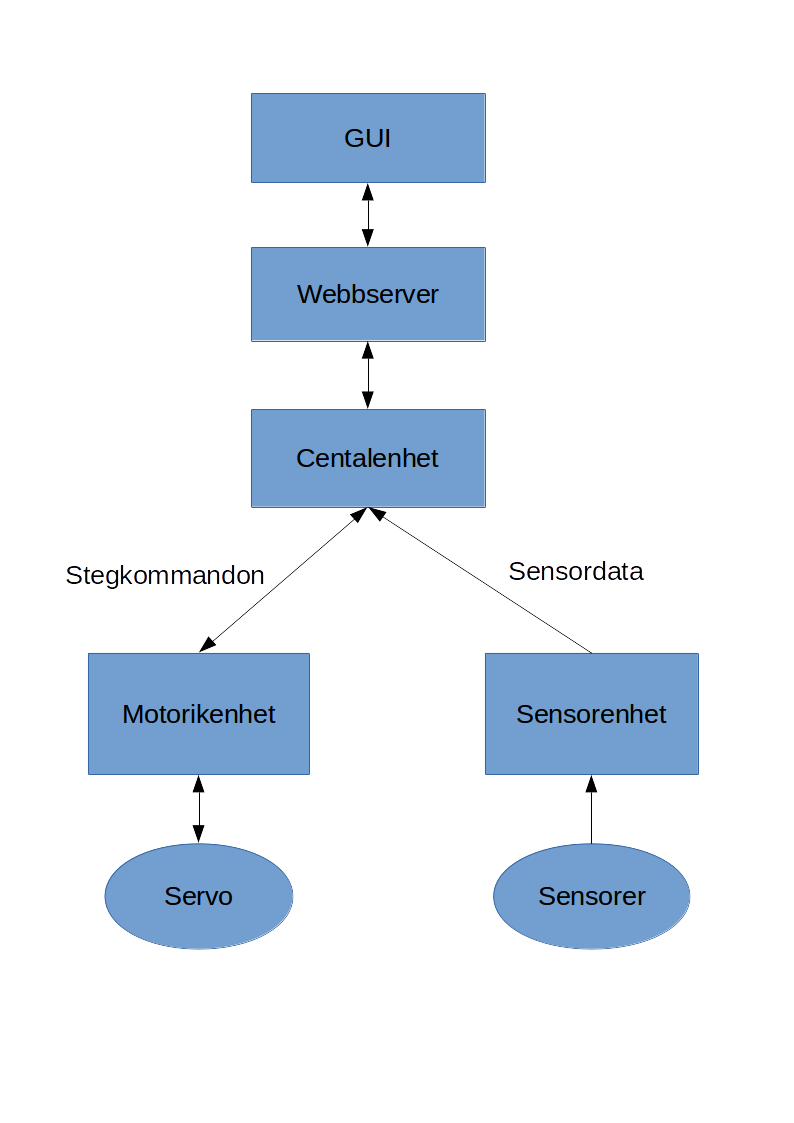
\includegraphics[width=0.8\linewidth]{images/overview.png}
		\caption{Översikt av systemet}
		\label{fig:images/overview}
	\end{figure}
	\subsection{Grov beskrivning av produkten}
	Systemet ska innehålla tre enheter. En centralenhet för kommunikation med en dator,
	en motorikenhet som sköter hur benen rör sig och en sista enhet för sensorer.
	Centralenheten är även den enhet som tar beslut och kommunicerar med de 
	andra enheterna. 

	\subsection{Produktkomponenter}
	I leveransen ska det ingå en autonom sexbent robot med tillhörande GUI som kan 
	användas för att styra roboten manuellt. Teknisk dokumentation och demonstration 
	ingår även. 
	\subsection{Beroenden  till andra system}
	Det beroende som finns är centralenhetens Wi-Fi-kommunikation som används för 
	att kommunicera med en dator.
	\subsection{Ingående delsystem}
	1. Centralenheten
	2. Motorikenhet
	3. Sensorenhet
	\subsection{Avgränsningar}
	\textbf{text}
	\subsection{Designfilosofi}
	\textbf{text}
	\subsection{Generella krav på hela systemet}

	%Generella krav på systemet
	\begin{table}[h!]
		\label{tab:label}
		\begin{tabularx}{\textwidth}{|l|l|X|l|}
		\hline
			\textbf{Krav nr} & \textbf{Förändring} & \textbf{Kravtext} & \textbf{Prioritet} 
				\\ \hline
	
			1 & original & Roboten ska autonomt kunna navigera sig igenom tvävlingsbanan & 1
					\\ \hline

			2 & original & Det ska finnas en knapp på roboten eller på GUIt som startar
				roboten i tävlingen & 1
				\\ \hline

			3 & original & Roboten ska gå att styra manuellt via en WiFi-länk& 1
				\\ \hline
		
			4 & original & Robotens sensordata ska gå att läsa med en dator via Wi-Fi & 1
				\\ \hline

			5 & original & Robotens styrbeslut ska gå att läsa med en dator via Wi-Fi & 1
				\\ \hline
		\end{tabularx}
	\end{table}

	%%%%%%%%%%%%%%%%%%%%%%%%%%%%%%%%%%%%%%%%%%%%%%%%%%%%%%%%%%%%%%%%%%%%%%%%%%%%%%%%%
	%						Centralenhet
	%%%%%%%%%%%%%%%%%%%%%%%%%%%%%%%%%%%%%%%%%%%%%%%%%%%%%%%%%%%%%%%%%%%%%%%%%%%%%%%%%
	\section{Delsystem centralenhet}
	Centralenheten ska styra alla andra delsystem i konstruktionen, samt sköta
	kommunikation till omvärlden via bland annat Wi-Fi. Denna utgörs av en Raspberry
	Pi, som är en passande dator då den har inbyggd hårdvara för WiFi och Wi-Fi samt
	ett operativsystem, som gör att programmering kan ske på en relativt hög nivå.
	\subsection{Inledande beskrivning av centralenhet}
	\textbf{table}
	\subsection{Gränssnitt}
	\begin{table}[h!]
		\label{tab:label}
		\begin{tabularx}{\textwidth}{|l|l|X|l|}
			\hline
			\textbf{Krav nr} & \textbf{Förändring} & \textbf{Kravtext} & \textbf{Prioritet} 
				\\ \hline

			1 & original & Centralenheten ska kunna kommunicera med en dator via Wi-Fi. & 1
				\\ \hline

			2 & original & Centralenheten ska kunna ta emot och behandla data från 
				sensorenheten.& 1
				\\ \hline

			3 & original & Centralenheten ska kunna ta emot, behandla och skicka 
				information  till motorikenheten& 1
				\\ \hline


		\end{tabularx}
	\end{table}

	\subsection{Funktionella krav för centralenhet}
	\begin{table}[h!]
		\label{tab:label}
		\begin{tabularx}{\textwidth}{|l|l|X|l|}
			\hline
			\textbf{Krav nr} & \textbf{Förändring} & \textbf{Kravtext} & \textbf{Prioritet} 
				\\ \hline

			4 & original & Centralenheten ska kuna hålla koll på sin position i labyrinten 
				med hjälp av sensorerna & 2
				\\ \hline
		\end{tabularx}
	\end{table}


	%%%%%%%%%%%%%%%%%%%%%%%%%%%%%%%%%%%%%%%%%%%%%%%%%%%%%%%%%%%%%%%%%%%%%%%%%%%%%%%%%
	%						Centralenhet
	%%%%%%%%%%%%%%%%%%%%%%%%%%%%%%%%%%%%%%%%%%%%%%%%%%%%%%%%%%%%%%%%%%%%%%%%%%%%%%%%%

	\section{Centralenhet}
	\textbf{text}
	\subsection{Inledande beskrivning av centralenhet}
	\textbf{table}
	\subsection{Gränssnitt}
	\textbf{table}
	\subsection{Designkrav}
	\textbf{table}
	\subsection{Funktionella krav för centralenhet}


	\section{Centralenhet}
	\textbf{text}
	\subsection{Inledande beskrivning av centralenhet}
	\textbf{table}
	\subsection{Gränssnitt}
	\textbf{table}
	\subsection{Designkrav}
	\textbf{table}
	\subsection{Funktionella krav för centralenhet}
	%%%%%%%%%%%%%%%%%%%%%%%%%%%%%%%%%%%%%%%%%%%%%%%%%%%%%%%%%%%%%%%%%%%%%%%%%%%%%%%%%
	%						Extrakrav
	%%%%%%%%%%%%%%%%%%%%%%%%%%%%%%%%%%%%%%%%%%%%%%%%%%%%%%%%%%%%%%%%%%%%%%%%%%%%%%%%%
	\section{Prestandakrav}
	\textbf{table}
	\section{Krav på vidareutveckling}
	\textbf{table}
	\section{Tillförlitlighet}
	\textbf{table}
	\section{Leveranskrav och  delleveranser}
	\textbf{table}
	\section{Dokumentation}
	\textbf{table}
	\section{Kvalitetskrav}
	\textbf{table}
	\section{Underhållsbarhet}
	\textbf{table}
	\section{Referenser}
	\textbf{table}







\end{document}




%%%%%%%%%%%%%%%%%%%%%%%%%%%%%%%%%%%%%%%%%%%%%%%%%%%%%%%%%%%%%%%%%%%%%%%%%%%%%%%%%
%						Templates
%%%%%%%%%%%%%%%%%%%%%%%%%%%%%%%%%%%%%%%%%%%%%%%%%%%%%%%%%%%%%%%%%%%%%%%%%%%%%%%%%

\iffalse
	\begin{table}[h!]
		\label{tab:label}
		\begin{tabularx}{\textwidth}{|l|l|X|l|}
		\hline
		\textbf{Krav nr} & \textbf{Förändring} & \textbf{Kravtext} & \textbf{Prioritet} 
		\\ \hline
	
		1 & original & Roboten ska autonomt kunna navigera sig igenom tvävlingsbanan & 1
		\\ \hline
		\end{tabularx}
	\end{table}
\fi
